\chapter{Visualization Tools}
\label{cpt:tools}

The main contribution of this project automatic methods for visualizing how a webcam
scene varies, and how we can understand the most important variations.  In most natural
scenes, we notice changes in lighting, weather, and camera conditions which are interesting,
but fail to describe the typical behavior of a scene.  The goal of these tools is to learn 
these variations and to point out changes separate from them.  PCA is a commonly used too, and
captures a linear model of consistent image variations.

\section{Setup}

\subsection{Temporal Narrowing}

\subsection{Sky Mask}

In many outdoor scenes, even when narrowed to a particular time of day, the most difficult image
variation to characterize is the sky.  PCA has a difficult time learning changes in sunlight, clouds,
and other characteristics of the sky, so this difficulty causes

Fortunately, it is fairly easy to learn which religions of an image are most affected by this challenge.

\begin{figure}
	\centering
	\subfigure[]{
		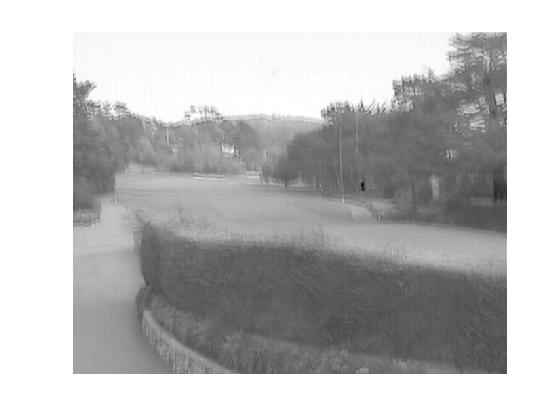
\includegraphics[width=0.45\textwidth]{figures/2skyPCA.jpg}
	\label{fig:carsNoGradient}
	}
	\subfigure[]{
		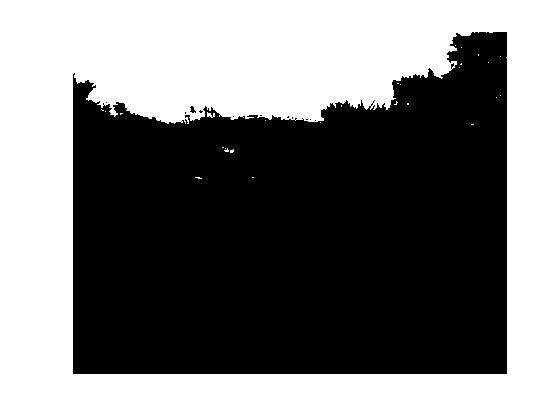
\includegraphics[width=0.45\textwidth]{figures/2skyMask.jpg}
	\label{fig:carsGradient}
	}
		\caption[Learning a sky mask for a webcam scene.]{Figure \ref{fig:2skyPCA} shows the first PCA component of a webcam scene.  By adding or subtracting this component, we control how dark or how light the sky is. Figure \ref{fig:2skyMask} shows that a simple threshholding of this image effectively segments the sky from the rest of the image.}
\end{figure}

\subsection{Gradient Image}

A webcam images are very high-dimensional - a typical 320 x 240 gray scale image has 76,800 pixels, each of
which is a value from 0 to 255.  One way to simplify this space without affecting the size of the image is to
look at the gradient magnitude images of a scene.


\begin{figure}
	\centering
	\subfigure[]{
		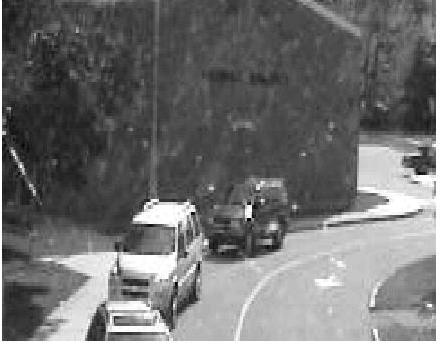
\includegraphics[width=0.45\textwidth]{figures/194cars.jpg}
	\label{fig:carsNoGradient}
	}
	\subfigure[]{
		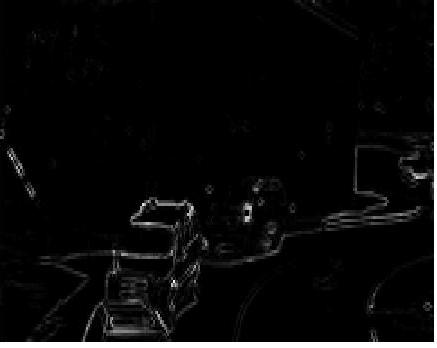
\includegraphics[width=0.45\textwidth]{figures/194carsGradient.jpg}
	\label{fig:carsGradient}
	}
		\caption[Focusing on object edges with gradient magnitude images.]{Figure \ref{fig:carsNoGradient} shows a grayscale webcam image. Figure \ref{fig:carsGradient} shows the gradient magnitude image of that frame.  Notice the noise is mostly removed and the edges are highlighted.}
\end{figure}

\section{Visualizations}

In this section, we present several tools to visualize the webcam scene based on criteria we will discuss in the next section.

\subsection{Image Montage}

\subsection{Intelligent Image Montage}

\subsection{Two-dimensional Explorer}

Using a simple GUI, we can explore a webcam scene in two dimensions.


\section{Criteria}

Once webcam scenes are projected onto a PCA basis, there are many different ways to analyze the results.
In this section, we will present several different criteria for evaluating an appearance model of a scene,
the meaning behind each criteria, and results.

\subsection{PCA coefficient vector magnitude}

For each image in a scene, PCA gives a vector of coefficients that correspond to the best linear combination
of basis images to reconstruct that image.  From this vector, we can assign each image a score equal to the
magnitude of this vector.  This gives

\subsection{Residual Error}

% figure of subplot with image, reconstruction, and residual



\subsection{Variance Model}

We can estimate the variance image of a webcam scene by summing the residual images.

% figure with variance image, and some zScores

\subsection{Probabilistic}

We can also try to learn about an image reconstruction by treating its residual image as samples from an 
underlying probability density function.

% figure showing different residual histograms

\begin{enumerate}
\item{\textbf{Normal Distribution Likelihood}}

The most obvious way to do this is to treat each residual image pixel as a sample from a normal distribution.  We can easily estimate the mean and variance of this PDF and then 

\item{\textbf{Laplacian Distribution Likelihood}}

Many of the residual images have a majority of pixels that are very close zero.  This causes the histogram to look
very similar to a laplacian distribution.

\item{\textbf{Kurtosis}}

\item{\textbf{Skewness}}

\end{enumeration}


